\documentclass[11pt,fullpage]{article}
%\usepackage{multicol,wrapfig,amsmath,subfigure}
\usepackage{amsmath}
\usepackage{amsfonts,amssymb}
\usepackage{ mathrsfs }
\usepackage{amsthm}
\usepackage{graphics,graphicx}
\usepackage{hyperref}
\usepackage{ stmaryrd }
\usepackage[right = 2.5cm, left=2.5cm, top = 2.5cm, bottom =2.5cm]{geometry}
\pagestyle{plain}
\def\urlfont{\DeclareFontFamily{OT1}{cmtt}{\hyphenchar\font='057}
	\normalfont\ttfamily \hyphenpenalty=10000}

\newcommand*{\plogo}{\fbox{$\mathcal{PL}$}}
\newcommand{\norm}[1]{\|#1\|}
\newcommand{\innprod}[1]{\langle #1 \rangle}
\newcommand{\Tau}{\mathcal{T}}
\newcommand{\lap}{\Delta}
\newcommand{\problem}[1]{\paragraph{Problem #1}}
%\input macros
\newcommand{\deriv}{\mbox{d}}
\newcommand{\Real}{\mathbb R}
\newcommand{\eps}{\epsilon}
\newcommand{\Complex}{\mathbb C}
\newcommand{\abs}[1]{\left\vert#1\right\vert}
\newcommand{\set}[1]{\left\{#1\right\}}
\newcommand{\subheading}[1]{\noindent \textbf{#1}}
\newcommand{\grad}{\nabla}
\newcommand{\diver}{\textup{div} }
\newcommand{\jump}[1]{[#1]}
\newcommand{\limit}[2]{\lim_{#1 \rightarrow #2}}
\newcommand{\mollify}[1]{ \mathcal{J}_\epsilon #1 }
\newcommand{\conv}[2]{#1 \ast #2}
\newcommand{\D}{D}
\newcommand{\K}{\mathcal{K}}
\newcommand{\C}{\mathcal{C}}
\newcommand{\Torus}{\mathbb{T}}
\newcommand{\Integer}{\mathbb{Z}}
\newcommand{\Naturals}{\mathbb{N}}
\newcommand{\ineqtext}[1]{ ^{\text{\tiny #1}}}
\newcommand{\F}{\mathcal{F}}
\newcommand{\bx}{\mathbf{x}}
\newcommand{\by}{\mathbf{y}}
\newcommand{\intab}{\int_{a}^{b}}
\newcommand{\intom}{\int_{\Omega}}
\newcommand{\Ltwo}{{L^2}}
\newcommand{\Ltwoom}{{L^2(\Omega)}}
\newcommand{\Linf}{{L^\infty}}
\newcommand{\Linfom}{{L^\infty(\Omega)}}
\renewcommand{\i}{{i}}
\newcommand{\ip}{{i+1}}
\newcommand{\ipp}{{i+2}}
\newcommand{\im}{{i-1}}
\newcommand{\imm}{{i-2}}
\renewcommand{\j}{{j}}
\newcommand{\jp}{{j+1}}
\newcommand{\jpp}{{j+2}}
\newcommand{\jm}{{j-1}}
\newcommand{\jmm}{{j-2}}
\newcommand{\n}{{n}}
\newcommand{\np}{{n+1}}
\newcommand{\npp}{{n+2}}
\newcommand{\nm}{{n-1}}
\newcommand{\nmm}{{n-2}}

%Nancy's macros
\newcommand{\reg}[1]{#1^\epsilon}
\newcommand{\Lpr}[1]{L^{#1}(\mathbb{R}^n)}
\newcommand{\Lp}[1]{L^{#1}(\Omega)}
\newcommand{\intreal}[1]{\int_{\mathbb{R}^{#1}}\hspace{-8pt}}
\newcommand{\modenergy}{\mathcal{E}_H}
\newcommand{\ball}{B_n}
\newcommand{\balltime}{B_n\times [0,T]}

\newtheorem{theorem}{Theorem}
\theoremstyle{lemma}
\newtheorem{prop}{Proposition}
\newtheorem{proposition}{Proposition}
\newtheorem{corollary}{Corollary}
\theoremstyle{definition}
\newtheorem{definition}{Definition}
\newtheorem{exercise}{Exercise}
\newtheorem{algorithm}{Algorithm}
\newtheorem{question}{Question}
%\theoremstyle{remark}
\newtheorem{remark}{Remark}
\newtheorem{rmk}{Remark}
\newtheorem{example}{Example}
\theoremstyle{lemma}
\newtheorem{lemma}{Lemma}
\allowdisplaybreaks

\begin{document}
	
\begin{center}
	\textbf{\Large{Scientific Computation of Two--Phase Ferrofluid Flows}}
	\\
	\textbf{\Large{AMSC 664}} \\ 
	\textbf{\large{Gareth Johnson}}\\
	\textbf{\large{Faculty Adviser: Ricardo Nochetto}}
	\\
	\today
\end{center}

\section{Introduction}
A ferrofluid is a liquid which becomes magnetized when under the effect of a magnetic field. A ferrofluid is a colloid of nanoscale ferromagnetic particles suspended in a carrier fluid such as oil, water, or an organic solvent. Due to their ability to be controlled by external magnetic fields, ferrofluids are used in a wide application of control based problems. Ferrofluids were first used to pump rocket fuel once a spacecraft entered a weightless environment \cite{Rocket}. Commercial uses of ferrofluids include applications in vibration damping, sensors, and acoustics \cite{CommercialAppl}. A more recent area of research is magnetic drug targeting, where drugs are injected and guided using magnetic fields to their specific destination \cite{DrugTarg:1, DrugTarg:2, DrugTarg:3}. A final application worth mentioning is the construction of adaptive deformable mirrors, which can be viewed as a shape optimization problem \cite{FerroMirror:1, FerroMirror:2, FerroMirror:3}. 

For one phase ferrofluid flows, there are two primary PDE models which mathematically describe the behavior of a ferrofluid under the effects of a magnetic field referred to by the names of their creators; the Rosensweig model \cite{Rosensweig} and the Shliomis model \cite{Shliomis}. Both models are current research areas, with existence of global weak solutions and local existence of strong solutions being recent results \cite{PDEResults:1,PDEResults:2, PDEResults:3, PDEResults:4}. However, these models do not describe two--phase ferrofluid flows, where one phase has magnetic properties and the other does not. While work has been done to create interface conditions for two--phase flows in the sharp interface regime \cite{SharpInter:1, SharpInter:2}, there is not an established PDE model which describes two--phase ferrofluid flows.

Using numerical analysis and scientific computation, new models can be developed through trial and error. To this extent, various computational methods have been used in order to numerically simulate various phenomenon of two--phase ferrofluid flows. For stationary phenomena, Tobiska and collaborators have devised numerical and physical experiments investigating the free surface of ferrofluids using a sharp interface approach \cite{Tob:1, Tob:2, Tob:3}. In \cite{Numerics:1, Numerics:2}, Volume of Fluid methods are used to numerically investigate non--stationary phenomena, such as the field induced motion of a ferrofluid droplet and the formation process of ferrofluid droplets respectively. 

An important issue with these techniques is that their numerical implementations, stability, and convergence are not explored. To this end, Nochetto and collaborators developed a model for two--phase ferrofluid flow and devised an energy stable numerical scheme \cite{DiffuseInterface}. The model presented was not derived but instead was assembled by selecting specific components from existing models and standard assumptions. This was done to create a simple model, focusing on a minimal number of constitutive parameters and coupled PDEs, that still captured the basic phenomena of two--phase ferrofluids. Below, we present the model in full and then summarize the derivation of each component and define all variables and parameters.

The model considers a two--fluid system, consisting of a ferrofluid and a non--ferromagnetic one, on a bounded convex polygon/polyhedron domain $\Omega\subset \Real^d$ ($d=2$ or $3$) with boundary $\Gamma$. The evolution of the system is given by the following set of equations in strong form in $\Omega$
\begin{subequations}\label{Model}
	\begin{align}
	\label{Cahn-Hilliard:1}\theta_t + \diver(\mathbf{u}\theta) + \gamma \lap \psi &= 0,\\
	\label{Cahn-Hilliard:2}\psi - \eps \lap \theta + \frac{1}{\eps}f(\theta) &= 0,\\
	\label{Advection-Reaction}\mathbf{m}_t + (\mathbf{u}\cdot \grad)\mathbf{m}&=-\frac{1}{\mathscr{T}}(\mathbf{m} - \varkappa_\theta\mathbf{h}),\\
	\label{MagScalarPot}-\lap \varphi &=\diver(\mathbf{m}-\mathbf{h}_a),\\
	\label{NavierStokes}\mathbf{u}_t + (\mathbf{u}\cdot\grad)\mathbf{u} - \diver (\nu_\theta \mathbf{T(u)}) + \grad p &= \mu_0(\mathbf{m}\cdot \grad)\mathbf{h} + \frac{\lambda}{\eps}\theta\grad \psi,\\
	\label{DivFree}\diver \mathbf{u} &= 0,
	\end{align}
\end{subequations}
for every $t\in[0,t_F]$, where $\mathbf{T(u)}=\frac{1}{2}(\grad \mathbf{u} + \grad\mathbf{u}^T)$ denotes the symmetric gradient and $\mathbf{h}=\grad \varphi$. The system (\ref{Model}) is supplemented with the boundary conditions
\begin{equation}\label{ModelBC}
	\partial_\eta \theta = \partial_\eta\psi = 0,\quad \mathbf{u}=0,\quad\text{and}\quad \partial_\eta\varphi = (\mathbf{h}_a - \mathbf{m})\cdot\eta \quad \text{on }\Gamma.
\end{equation}

The position of each fluid is tracked using a phase variable $\theta$, which makes the model a diffuse--interface type. The phase variable $\theta$ takes values in $[-1,1]$, where $\theta = \pm 1$ denotes a pure concentration of a single fluid and values in $(-1,1)$ denotes the interface between the fluids. The evolution of the phase variable is governed by the Cahn--Hilliard equation, given by (\ref{Cahn-Hilliard:1}) and (\ref{Cahn-Hilliard:2}), where $0< \eps <<1$ is the interface thickness, $\gamma>0$ is the (constant) mobility, $\psi$ is the chemical potential, $f(\theta)=F'(\theta)$ and $F(\theta)$ is the truncated double well potential
\begin{equation}\label{DoublePotent}
	F(\theta) = \begin{cases}
	(\theta + 1)^2 &\text{if }\theta\in(-\infty,-1]\\
	\frac{1}{4}(\theta^2 - 1)^2 &\text{if }\theta\in[-1,1]\\
	(\theta -1)^2 &\text{if }\theta\in[1,+\infty).
	\end{cases}
\end{equation}

The evolution of the magnetization $\mathbf{m}$, which is induced by a magnetic field $\mathbf{h}$ defined as the gradient of a magnetic potential $\varphi$, is given by the simplified advection--reaction equation (\ref{Advection-Reaction}). In (\ref{Advection-Reaction}), $\mathscr{T}$ is the relaxation time of the ferrofluid and $\varkappa_\theta$ is the magnetic susceptibility of the phase variable. Defining $\varkappa_0>0$ to be the magnetic susceptibility of the ferrofluid and setting the non--magnetic fluid to have zero magnetic susceptibility, we have that $\varkappa_\theta$ is a Lipschitz continuous function of $\theta$ satisfying $0\leq \varkappa_\theta \leq \varkappa_0$. The magnetic field $\mathbf{h}$ is the sum of a smooth harmonic applied magnetizing field $\mathbf{h}_a$ (i.e. $\diver \mathbf{h}_a = 0,\quad \text{curl}\mathbf{h}_a=0$) and a de--magnetizing field $\mathbf{h}_d$. It is modeled using a scalar potential $\varphi$ which satisfies $\mathbf{h} = \grad \varphi$ and equation (\ref{MagScalarPot}). 

Finally, the velocity--pressure pair $(\mathbf{u}, p)$ are given by a simplified Navier--Stokes equation (\ref{NavierStokes}) coupled with an incompressibility condition (\ref{DivFree}). In (\ref{NavierStokes}), $\nu_\theta$ is the viscosity of the phase variable, $\mu_0$ is the constitutive parameter related to the Kelvin force, and $\frac{\lambda}{\eps}\theta\grad \psi$ is the capillary force. Defining $\nu_w, \nu_f$ to be the viscosities of the non--magnetic fluid and the ferrofluid respectively, we have that $\nu_\theta$ is a Lipschitz continuous function of $\theta$ satisfying
$$
	0 < \min\set{\nu_w, \nu_f} \leq \nu_\theta \leq \max\set{\nu_w, \nu_f}.
$$

In order to solve system (\ref{Model}), the following numerical scheme is proposed in \cite{DiffuseInterface}. Define $K>0$ to be the number of time steps, with uniform time step $\tau = T/K>0$. Define the backwards difference operator $\delta$:
$$
	\delta f^k = f^k - f^{k-1}.
$$
Define the following finite dimensional subspaces $\mathbb{G}_h\subset H^1(\Omega), \mathbb{Y}_h\subset H^1(\Omega), \mathbb{M}_h\subset L^2(\Omega), \mathbb{X}_h\subset H^1(\Omega), \mathbb{U}_h\subset H^1_0(\Omega),$ and $\mathbb{P}_h\subset L^2(\Omega)$ that will approximate the phase field, chemical potential, magnetization, magnetic potential, velocity, and pressure respectively. In the context of finite elements, the above spaces are parameterized by the meshsize $h$. The pair of spaces $(\mathbb{U}_h, \mathbb{P}_h)$ are assumed to satisfy a uniform inf--sup condition
\begin{equation}
\inf_{0\neq Q\in\mathbb{P}_h}\sup_{0\neq \mathbf{V}\in\mathbb{V}_h}\frac{(\diver \mathbf{V}, Q)}{\norm{Q}_{\Ltwo}\norm{\mathbf{V}}_\Ltwo}\geq \beta^*,
\end{equation}
with $\beta^*>0$ independent of $h$. Introduce a suitable discretization of the trilinear form for the convective term in the Navier--Stokes equation:
$$
\mathcal{B}_h(\cdot,\cdot,\cdot):\mathbb{U}_h\times\mathbb{U}_h\times\mathbb{U}_h\to\Real.
$$
Additionally, introduce a suitable discretization of the trilinear form for the convective term of (\ref{Advection-Reaction}) and the Kelvin force in (\ref{NavierStokes}):
$$
\mathcal{B}_h^m(\cdot,\cdot,\cdot):\mathbf{U}_h\times\mathbf{M}_h\times\mathbf{M}_h\to\Real.
$$
For given smooth initial data $\set{\Theta^0, \mathbf{M}^0,\mathbf{U}^0}$, compute $\set{\Theta^k, \Psi^k, \mathbf{M}^k, \Phi^k, \mathbf{U}^k, {P}^k}\in \mathbb{G}_h\times \mathbb{Y}_h\times \mathbb{M}_h\times\mathbb{X}_h\times\mathbb{U}_h\times\mathbb{P}_h$ for every $k\in\set{1,...,K}$ that solves
\begin{subequations}\label{NumScheme}
	\begin{align}
	\label{NumScheme:1}\bigg(\frac{\delta\Theta^k}{\tau}, \Lambda\bigg) - (\mathbf{U}^k\Theta^{k-1}, \grad\Lambda) - \gamma(\grad \Psi^k, \grad \Lambda)&=0,\\
	\label{NumScheme:2}(\Psi^k, \Upsilon) + \eps(\grad \Theta^k, \grad \Upsilon) + \frac{1}{\eps}(f(\Theta^{k-1}), \Upsilon) + \frac{1}{\eta}(\delta\Theta^k, \Upsilon) &= 0,\\
	\label{NumScheme:3}\bigg(\frac{\delta\mathbf{M}^k}{\tau}, \mathbf{Z}\bigg) - \mathcal{B}_h^m(\mathbf{U}^k, \mathbf{Z}, \mathbf{M}^k) + \frac{1}{\mathscr{T}}(\mathbf{M}^k, \mathbf{Z}) &= \frac{1}{\mathscr{T}}(\varkappa_\theta\mathbf{H}^k, \mathbf{Z}),\\
	\label{NumScheme:4}(\grad\Phi^k, \grad X) &= (\mathbf{h}_a^k - \mathbf{M}^k, \grad X),\\
	\begin{split}
	\label{NumScheme:5}\bigg(\frac{\delta\mathbf{U}^k}{\tau}, \mathbf{V}\bigg) + \mathcal{B}_h(\mathbf{U}^{k-1}, \mathbf{U}^k, \mathbf{V}) + (\nu_\theta\mathbf{T(U}^k), \mathbf{T(V)}) - (P^k, \diver \mathbf{V}) &= \mu_0\mathcal{B}_h^m(\mathbf{V}, \mathbf{H}^k, \mathbf{M}^k)\\
	&\phantom{{}={}}+\frac{\lambda}{\eps}(\Theta^{k-1}\grad \Psi^k, \mathbf{V}),
	\end{split}\\
	\label{NumScheme:6}(Q, \diver\mathbf{U}^k) &= 0,
	\end{align}
\end{subequations}
for all $\set{\Lambda, \Upsilon, \mathbf{Z}, X, \mathbf{V}, Q}\in \mathbb{G}_h\times \mathbb{Y}_h\times \mathbb{M}_h\times\mathbb{X}_h\times\mathbb{U}_h\times\mathbb{P}_h$, where $\mathbf{H}^k=\grad \Phi^k$ and $\eta \leq \big(\max_\theta f'(\theta)\big)^{-1}$. The numerical scheme (\ref{NumScheme}) was proven to be energy--stable and locally solvable \cite{DiffuseInterface}. 

\section{Project Goal}
The main goal of the project was to develop a finite element code to solve two--phase ferrofluid flows using the numerical scheme (\ref{NumScheme}). In order to track progress made, the project was divided into the following four tasks. 
\begin{itemize}
	\item The first task was to develop code to solve the Cahn--Hilliard system (\ref{NumScheme:1})--(\ref{NumScheme:2}). In addition to solving the system, this task included adding functionality for adaptive mesh refinement/coarsening. This is because we are using the variable $\Theta$ in the definition of the Kelly error estimator \cite{ErrorInd}
	\begin{equation}\label{ErrorInd}
	\eta_T^2 = h_T\int_{\partial T}\abs{\bigg\llbracket\frac{\partial \Theta}{\partial \eta}\bigg\rrbracket}^2dS \quad \forall T\in\Tau_h,
	\end{equation}
	which will determine which elements are coarsened/refined. 
	
	\item The second task was to develop code to solve the Navier--Stokes system (\ref{NumScheme:5})--(\ref{NumScheme:6}).
	
	\item The third task was to develop code to solve the Magnetization system (\ref{NumScheme:3})--(\ref{NumScheme:4}). 
	
	\item The final task was to solve the overall scheme by combining the above solvers using a Picard--like iteration.
\end{itemize}
The solvers were to be developed in C++ and were to utilize the deal.II library \cite{AdaptiveMesh:1, DealII}. 

Due to the deal.II library having a steeper learning curve than initially expected, none of the above tasks had been started by the end of last semester. Thus, the plan for this semester was to progress through each solver one at a time, moving onto the next only after the solver was passing unit testing. Following this plan, I was successfully able to complete the first two tasks, i.e. the solvers for the Cahn--Hilliard and Navier--Stokes systems have been implemented and unit tested. Due to the amount of time remaining in the semester after completing these two tasks, Dr. Ricardo suggested that I attempt to combine the two solver in order to have implemented a two--phase fluid solver. However, at the time of writing this report the combined solver is still currently in development and the progress will be detailed in Section 3.

\section{Implementation Details}
\subsection{Adaptive Mesh Refinement/Coarsening}
deal.II already provides methods for adaptive mesh refinement/coarsening. Specifically, it provides a method to mark elements for refinement/coarsening based on D\"ofler marking. The procedure is as follows:
\begin{itemize}
	\item[1)] Compute the Kelly error estimator (\ref*{ErrorInd}) on each element.
	
	\item[2)] Order the elements based on their error estimator value from highest to lowest.
	
	\item[3)] Compute the set of elements $M$, starting with elements with the highest error, such that the sum of their error makes up 55 percent of the total error. The elements in $M$ are then marked for refinement.
	
	\item[4)] Compute the set of elements $N$, starting with elements with the lowest error, such that the sum of the error makes up 5 percent of the total error. The elements in $N$ are then marked for coarsening.
	
	\item[5)] Refine/coarsen the mesh and then transfer the solution from the old mesh to the new mesh.
\end{itemize}
In order to ensure the number of elements does not grow without bound, we imposed that an element can only be refined up to a maximum of 5 times. This maximum number of refinements was chosen such that the interface appeared to be adequately resolved for a flat profile with $\eps = .001$. This particular value for the interface thickness was inspired by numerical experiments performed in \cite{DiffuseInterface}. 

Additionally, we perform adaptive mesh refinement/coarsening on the initial condition. This is because the initial mesh, as proposed in \cite{DiffuseInterface}, is too coarse for the interface of the initial condition to be resolved. Thus, by refining/coarsening on the initial condition we can ensure that from the beginning of the simulation that the interface is adequately resolved. Specifically, we allow for a the initial data to undergo 20 iterations of adaptive mesh refinement/coarsening. This number of initial iterations was determined by simply examining output of a flat profile for various numbers of refinement/coarsening iterations.

Finally, this adaptive procedure is currently run ever 5 time steps of the Cahn--Hilliard solver. This value is again taken from \cite{DiffuseInterface} and we note here that this value should really depend on the time scale of the dynamics of the Cahn--Hilliard equation. But since adaptive mesh refinement/coarsening is not the focal point of the project, we use the simpler approach of running the procedure every set number of time steps.

\subsection{Cahn--Hilliard Solver}
Consider the following rearranged version of the Cahn--Hilliard system (\ref{NumScheme:1})--(\ref{NumScheme:2})
\begin{align*}
\bigg(\Theta^k, \Lambda\bigg) - \tau\gamma(\grad \Psi^k, \grad \Lambda)&=\bigg(\Theta^{k-1}, \Lambda\bigg) + \tau(\mathbf{U}^k\Theta^{k-1}, \grad\Lambda),\\
(\Psi^k, \Upsilon) + \eps(\grad \Theta^k, \grad \Upsilon) + \frac{1}{\eta}(\Theta^k, \Upsilon) &= \frac{1}{\eta}(\Theta^{k-1}, \Upsilon)-\frac{1}{\eps}(f(\Theta^{k-1}), \Upsilon).\\
\end{align*}
This leads to the following block matrix form
$$\begin{pmatrix}
M & -\tau\gamma K \\
\eps K + \frac{1}{\eta}M & M
\end{pmatrix}
\begin{pmatrix}
\Theta^k\\
\Psi^k
\end{pmatrix} = 
\begin{pmatrix}
f\\
g
\end{pmatrix},
$$
where $M$ and $K$ are the usual mass and stiffness matrices and $f$ and $g$ are the respective right hand sides. We can eliminate the chemical potential $\Psi$ by adding $\tau\gamma KM^{-1}$ times the second row to the first row. Doing so yields the following reduced equation for the phase
$$
\bigg(M + \tau\eps\gamma KM^{-1}K + \frac{\tau \gamma}{\eta}K\bigg)\Theta^k = f + \tau \gamma KM^{-1}g.
$$
In order to help condition the system, we construct a preconditioner by simply replacing the inverse of $M$ by the inverse of the diagonal of $M$, i.e.
$$
	P = M + \tau\gamma\eps K\text{diag}(M)^{-1}K + \tau\frac{\gamma}{\eta}K.
$$
This choice was made as it was simple and easy to implement. Then the system is solved using GMRES with an incomplete LU preconditioner, which is a class provided by the deal.II library, of the matrix P. An important implementation detail is we never actually store the matrix
$$
M + \tau\eps\gamma KM^{-1}K + \frac{\tau \gamma}{\eta}K.
$$
This is because for the GMRES solver we only need to know its action on a vector. This is further used to compute the action of the matrix $M^{-1}$, which is also never explicitly computed. Instead we compute its action on a vector $x$ by solving the system
$$
	My = x
$$
iteratively using CG with an incomplete LU preconditioner. After solving for the phase, we can then solve for the chemical potential by solving the following system
$$
M \Psi^k = g - \bigg(\eps K + \frac{1}{\eta}M\bigg)\Theta^k
$$
using CG. 

\subsection{Navier--Stokes Solver}
The Navier--Stokes system (\ref{NumScheme:5})--(\ref{NumScheme:6}) can be rewritten into the following block matrix form
	$$\begin{pmatrix}
F & B^T \\
B & 0
\end{pmatrix}
\begin{pmatrix}
\mathbf{U}^k\\
P^k
\end{pmatrix} = 
\begin{pmatrix}
f\\
0
\end{pmatrix},
$$
where 
$$
F = \big(\mathbf{U}^k, \mathbf{V}\big) + \tau\mathcal{B}_h(\mathbf{U}^{k-1}, \mathbf{U}^k, \mathbf{V}) + \tau(\nu_\theta\mathbf{T(U}^k), \mathbf{T(V)}),
$$
$$
B = (Q, \diver\mathbf{U}^k),
$$
and 
$$
f = \big(\mathbf{U}^{k-1}, \mathbf{V}\big) + \tau\mu_0\mathcal{B}_h^m(\mathbf{V}, \mathbf{H}^k, \mathbf{M}^k) + \tau\frac{\lambda}{\eps}(\Theta^{k-1}\grad \Psi^k, \mathbf{V}).
$$
The trilinear form $\mathcal{B}_h$ is defined as the classical Temam modification of the convection term \cite{temam2001navier},
$$
	\mathcal{B}_h(\mathbf{U}, \mathbf{V}, \mathbf{W}) = \sum_{\Tau\in \Tau_h}\int_T (\mathbf{U}\cdot \grad)\mathbf{V}\cdot\mathbf{W} + \frac{1}{2}\diver\mathbf{U}\mathbf{V}\cdot\mathbf{W}.
$$
This trilinear form is consistent with the continuous trilinear form, as the second term vanishes if the velocity $\mathbf{U}$ is divergence free.
An ideal block preconditioner for the system would be
$$
P = \begin{pmatrix}
	F & 0\\
	B & -S
\end{pmatrix},
$$
where $S$ is the Schur Complement $S = B^TF^{-1}B$. This preconditioner is desirable as it has the property that
	$$
P^{-1}\begin{pmatrix}
F & B^T \\
B & 0
\end{pmatrix} = \begin{pmatrix}
F^{-1} & 0 \\
S^{-1}BF^{-1} & -S^{-1}
\end{pmatrix}\begin{pmatrix}
F & B^T \\
B & 0
\end{pmatrix} = \begin{pmatrix}
I & F^{-1}B^T \\
0 & I
\end{pmatrix},
$$
which is computationally easy to solve. However, this choice of preconditioner would require computing the inverse of various matrices, which is a numerically unstable operation. Thus, inspired by the block preconditioner proposed in Step--31 of the deal.II tutorials for solving the Boussinesq equation, we consider the following approximation for $P^{-1}$:
$$
	P^{-1} \approx \begin{pmatrix}
	\overset{\sim}{F}^{-1} & 0\\
	\overset{\sim}{S}^{-1}B\overset{\sim}{F}^{-1} & -\overset{\sim}{S}^{-1}
	\end{pmatrix},
$$
where $\overset{\sim}{F}^{-1}$ is computed using an inverse action, $\overset{\sim}{S}^{-1}$ is the Least Squares Commutator (LSC) \cite{Precond} defined as
$$
\overset{\sim}{S}^{-1} = \big(B\text{diag}(M)^{-1}B^T\big)^{-1}\big(B\text{diag}(M)^{-1}F\text{diag}(M)^{-1}B^T\big)\big(B\text{diag}(M)^{-1}B^T\big)^{-1},
$$
and $M$ is the mass matrix for the velocity.

In order to use the above approximation of $P^{-1}$ to solve our system using GMRES, a class was implemented which computes the action of the block preconditioner on a vector. This class is then called by the GMRES solver to precondition the above block system. Specifically, the class uses the following procedure to compute $Y = P^{-1}X$, where $X,Y$ are block vectors:
\begin{itemize}
	\item First, compute
	$$
	Y_0 = \overset{\sim}{F}^{-1}X_0.
	$$
	\item Second, in a temporary vector $N$ compute
	$$
	N = X_1 - BX_0 = X_1 - B\overset{\sim}{F}^{-1}X_0.
	$$
	\item Finally, compute
	$$
	Y_1 = \overset{\sim}{S}^{-1}N = \overset{\sim}{S}^{-1}\big(X_1 - B\overset{\sim}{F}^{-1}X_0\big).
	$$
\end{itemize}
Additionally, the block preconditioner uses an algebraic multigrid preconditioner (AMG) when using CG to solve for the inverse action of a matrix. The AMG preconditioner is used as a black box, using the same configuration as presented in the Step--31 tutorial of deal.II. This choice was made as it was computationally faster when compared to using the incomplete LU preconditioner used for matrix inverse actions in the Cahn--Hilliard solver.

\subsection{Two--phase Fluid Solver}
The two--phase fluid solver is the result of dropping the magnetization $\mathbf{M}$ and the magnetic field $\mathbf{H}$ from the numerical scheme \ref{NumScheme}, resulting in the numerical scheme
\begin{align*}
\bigg(\frac{\delta\Theta^k}{\tau}, \Lambda\bigg) - (\mathbf{U}^k\Theta^{k-1}, \grad\Lambda) - \gamma(\grad \Psi^k, \grad \Lambda)&=0,\\
(\Psi^k, \Upsilon) + \eps(\grad \Theta^k, \grad \Upsilon) + \frac{1}{\eps}(f(\Theta^{k-1}), \Upsilon) + \frac{1}{\eta}(\delta\Theta^k, \Upsilon) &= 0,\\
\bigg(\frac{\delta\mathbf{U}^k}{\tau}, \mathbf{V}\bigg) + \mathcal{B}_h(\mathbf{U}^{k-1}, \mathbf{U}^k, \mathbf{V}) + (\nu_\theta\mathbf{T(U}^k), \mathbf{T(V)}) - (P^k, \diver \mathbf{V}) &= \frac{\lambda}{\eps}(\Theta^{k-1}\grad \Psi^k, \mathbf{V})\\
(Q, \diver\mathbf{U}^k) &= 0.
\end{align*}
Implementation wise, the solver was created by combining the above two solvers with a Picard iteration to solve for the velocity at each time step. We consider the velocity to have converged if 
$$
	\norm{f - (F\mathbf{U} + B^T p)}_{l^2} \leq 10^{-5}\norm{f}_{l^2},
$$
which is the convergence criteria for the steady Navier--Stokes equations presented in \cite{Precond}. Due to the flow of the two fluid no longer being driven by a magnetic field, we drive the flow of the fluid by using a forcing function based on a forced solution for the velocity and pressure. However, when using this particular forcing the Picard iterate is currently not converging. More time will need to be spent in order to diagnose what is causing the Picard iteration to not converge. Due to this, the code will be present in the git repository but I do not consider it a deliverable due to the fact that it will need a good amount of work to get it into a functional state. It will be located in a folder marked NotWorking.


\section{Validation Methods}
All unit tests described below are in the testing folder in the git repository. These are slightly modified versions of the classes in the main source directory, with the modifications allowing for the automated tests to be ran. The Cahn--Hilliard and Navier--Stokes unit tests are executed from the test class called by UnitTesting.cpp. Below are descriptions of the unit tests as well as descriptions of the output showing that the unit tests are passing.

\subsection{Cahn--Hilliard Unit Tests}
The Cahn--Hilliard solver was verified with three unit tests. All three cases test the solver in "isolation" with $\mathbf{U} = 0$. The first unit test evaluates if the solver can resolve the interface of a stationary flat profile using adaptive refinement. This equates to specifying a flat profile as the initial condition and not having a forcing function. We expect that the mesh will be heavily refined around the interface and that the solution will stay stationary in time. The domain was taken to be $[0,0.6]\times [0,1]$ with 10 elements in the $x$--direction and 6 elements in the $y$--direction, which is the domain and initial mesh configuration specified in \cite{DiffuseInterface}. The initial condition for the flat profile was taken to be
$$
f(x, y) = \begin{cases}
-1 & y > .06\\
1 & \text{otherwise}
\end{cases},
$$
and the model parameters were chosen to be $\eps = .001$, $\gamma = .2$, $\eta = .000001$. Finally, the initial data was refined 20 times and the maximum level of refinement was 5. Below are plots of the initial condition on the refined mesh and the solution after $1000$ iterations at $t=1.0$.
\begin{figure}[!ht]
	\begin{minipage}{.4\paperwidth}
			\centering
			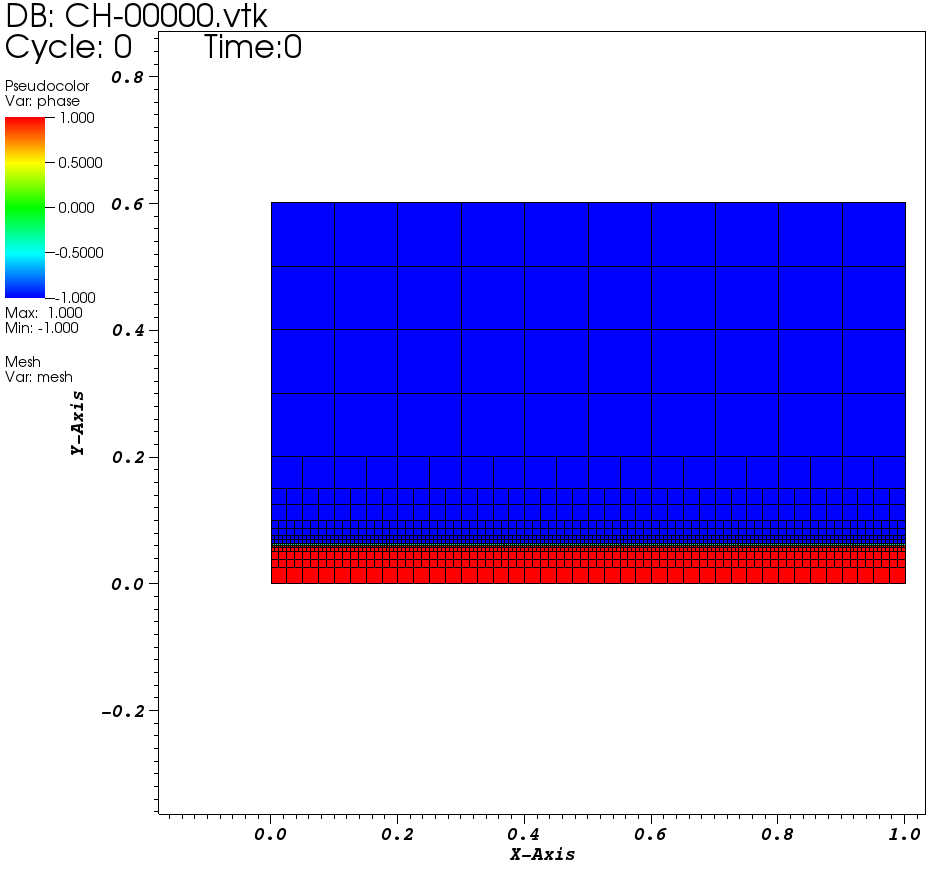
\includegraphics[scale=.9]{CHFlat1.png}
			\\Time step 0
	\end{minipage}%
	\begin{minipage}{.4\paperwidth}
			\centering
			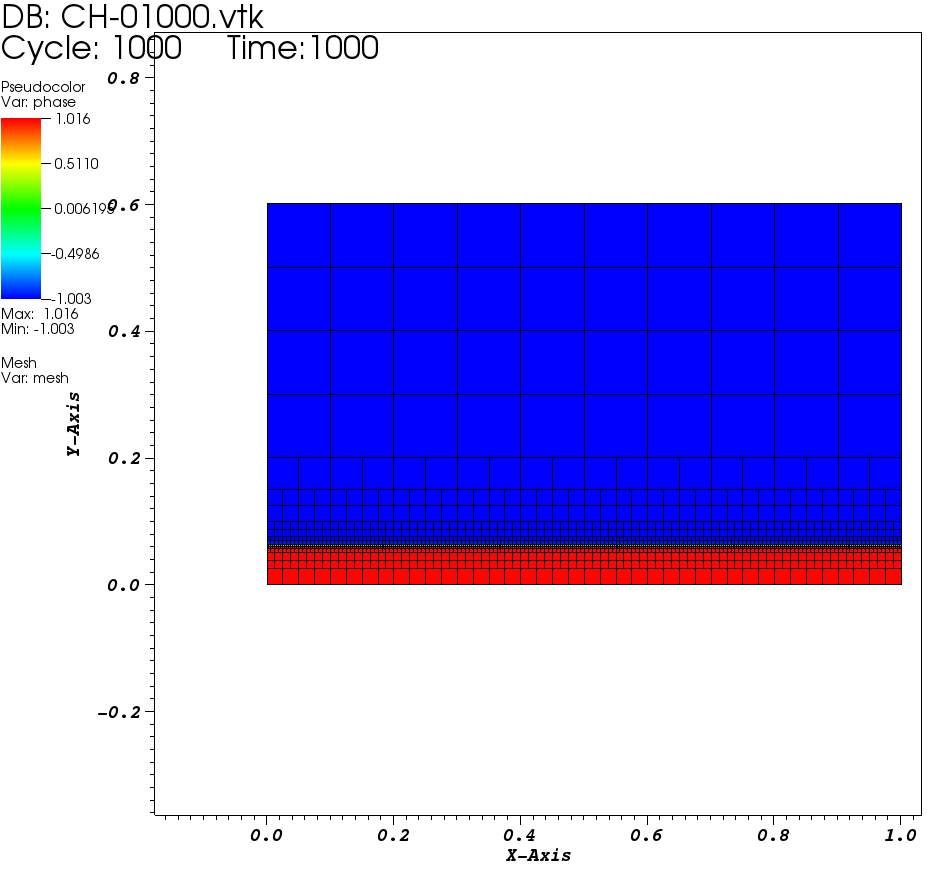
\includegraphics[scale=.9]{CHFlat2.png}
			\\Time step 1000
	\end{minipage}
\end{figure}\\
From the above plots we can see that the interface was heavily refined and that the solution remains constant in time, which is exactly what we expected.

The second unit test repeats the above but with the initial profile being a ball centered at $(0.5, 0.3)$ with radius $0.2$. This initial profile was chosen in order to verify that the interface could be resolved even when it was not aligned to the orientation of the mesh. The initial condition was defined as
$$
f(x, y) = \begin{cases}
-1 & (x,y)\in B((.5, .3), .2)\\
1 & \text{otherwise}
\end{cases},
$$
and the model parameters, domain, and refinement parameters remain the same as the first unit test. Below are plots of the initial condition on the refined mesh and the solution after $1000$ iterations at $t=1.0$.
\begin{figure}[ht!]
	\begin{minipage}{.4\paperwidth}
		\centering
		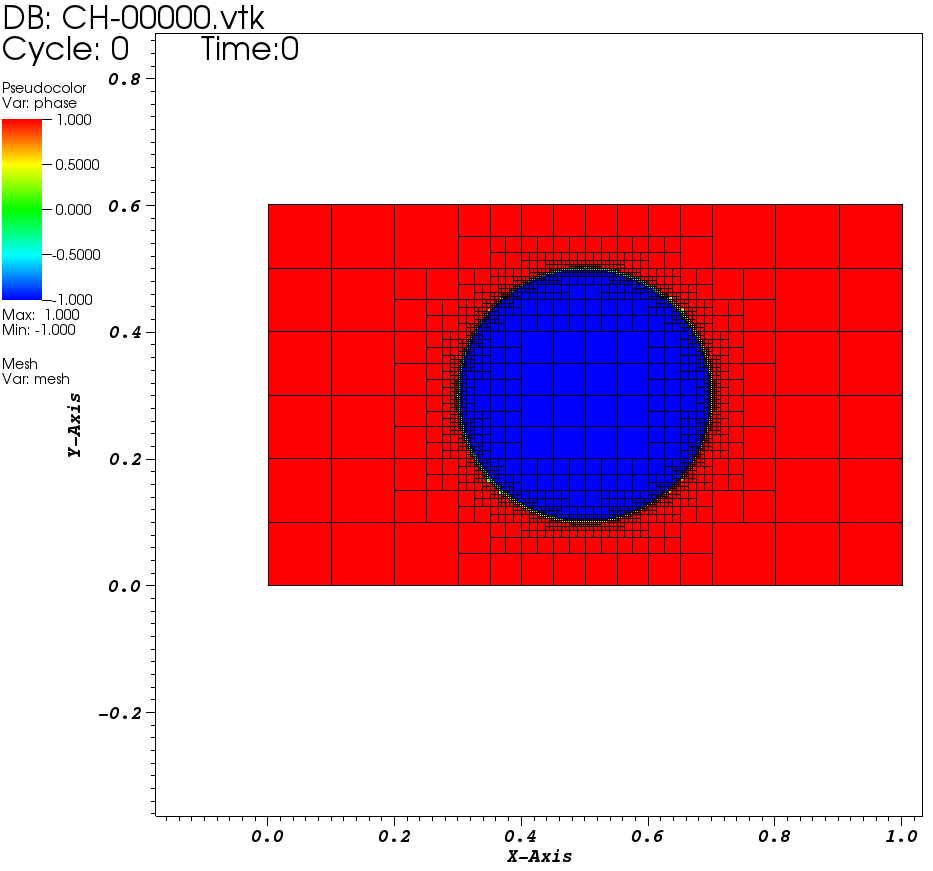
\includegraphics[scale=.9]{CHBall1.png}
		\\Time step 0
	\end{minipage}%
	\begin{minipage}{.4\paperwidth}
		\centering
		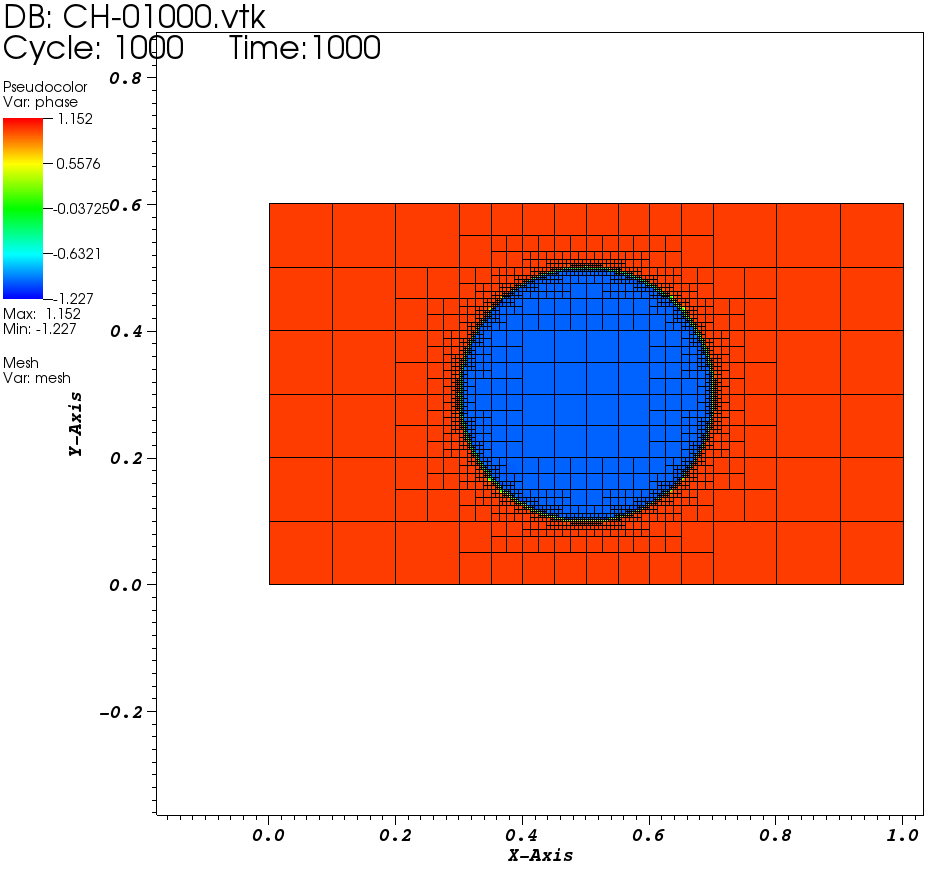
\includegraphics[scale=.9]{CHBall2.png}
		\\Time step 1000
	\end{minipage}
\end{figure}
Again, we can see that the initial mesh is heavily refined around the interface of the initial condition. However, there are intrinsic difficulties about trying to approximate a circle using a rectangular grid, which leads to the interface having rough edges in certain regions. Additionally, the error of the solution does not grow in time even though the coloring of the second plot does slightly change.

The final unit test verifies the solver by computing the error using a forced solution. This is achieved by choosing an analytic solution, computing and applying the appropriate forcing function to the system, and then solving the problem on a sequence of globally refined meshes. The domain was $[-1,1]^2$ and the analytic solution was chosen to be
$$
	f(x,y) = \cos(2\pi x)\cos(2\pi y).
$$
Unlike the previous unit tests, the thickness of the interface must be raised due to the fact that our chosen analytic solution does not naturally have an interface. Thus the model parameters used were $\eps = .2$, $\gamma = .2$, $\eta = .000001$. The $L^2$ and $H^1$--seminorm error were computed at iteration 1000 at $t=1.0$ on meshes with uniform refinement levels $2-6$.

\begin{figure}[!ht]
	\centering
	\begin{tabular}{|c|r|c|c|c|c|c|} \hline
		\multicolumn{2}{|c|}{n cells} & 
		\multicolumn{2}{|c|}{$H^1$-error} & 
		\multicolumn{2}{|c|}{$L^2$-error}\\ \hline
		2 & 16 & 4.264e+00 & Rate & 3.109e-01 &  Rate\\ \hline
		3 & 64 & 8.079e-01 &  2.40 & 2.658e-02 &  3.55\\ \hline
		4 & 256 & 2.038e-01 &  1.99 & 3.310e-03 &  3.01\\ \hline
		5 & 1024 & 5.104e-02 &  2.00 & 4.125e-04 &  3.00\\ \hline
		6 & 4096 & 1.277e-02 &  2.00 & 5.152e-05 &  3.00\\ \hline
	\end{tabular}
\end{figure}
\noindent From the above figure, we can see that the convergence rate has order 3 for the $L^2$ error and order $2$ for the $H^1$--seminorm error which is what we expect for $Q^2$ elements.

\subsection{Navier--Stokes Unit Test}
The Navier--Stokes solver was also verified by computing the error using a forced solution. Additionally, it tests the system in "isolation" with $\mathbf{\Theta} = \mathbf{\Psi} = \mathbf{M} = \mathbf{H} = 0$. The domain was $[0,1]^2$ and the forced solution was chosen to be
$$
\mathbf{u}(x,y,t) = \begin{pmatrix}
-2\pi\sin(t)\sin(\pi x)\sin(\pi y)\cos(\pi y)\\
2\pi\sin(t)\sin(\pi x)\cos(\pi x)\sin(\pi y)
\end{pmatrix}, \quad p(x,y,t) = \sin(2\pi(x - y) + t),
$$
as it is divergence free and obeys the no--slip boundary conditions. The model parameters used were $\mu = 1$, $\lambda = .05$, $\eps = .2$. The $L^2$ and $H^1$--seminorm error were computed at iteration 1000 at $t=2.0$ on meshes with uniform refinement levels $2-5$.
\begin{figure}[!ht]
	\centering
	\begin{tabular}{|c|r|c|c|c|c|} \hline
		\multicolumn{2}{|c|}{n cells} & 
		\multicolumn{2}{|c|}{$H^1$-error} & 
		\multicolumn{2}{|c|}{$L^2$-error}\\ \hline
		2 & 16 & 1.325e+00 &  Rate & 3.803e-02 & Rate\\ \hline
		3 & 64 & 3.393e-01 &  1.97 & 5.171e-03 & 2.88\\ \hline
		4 & 256 & 8.485e-02 &  2.00 & 1.254e-03 & 2.04\\ \hline
		5 & 1024 & 2.189e-02 &  1.95 & 1.064e-03 & 0.24\\ \hline
	\end{tabular}
\end{figure}
From the below figure, we can see that the $L^2$ error converges and that the $H^1$--seminorm has a convergence rate of order 2 which is the norm that is directly controlled by the finite element method.

In order to fix the convergence issues discussed in the final presentation, we found a simple bug in the way we were computing the forcing function. We simply were missing a factor of $0.5$ on the vector laplacian which is a consequence of that fact that for a divergence free velocity we have that
$$
	\diver(T(\mathbf{U})) = .5 \lap \mathbf{U}.
$$
Once this factor was added, the code started converging.

\subsection{Applied Magnetic Field Unit Test}
Last semester, a function was implemented which determines the value of the applied magnetic field at a point on the mesh given a set of magnetic dipoles with corresponding intensity values. This code is unit tested by choosing a known set of dipole locations and intensity values and then computing the analytic value of the magnetic field at various coordinates. We when compare the numerically computed values against the analytic values, with an error tolerance of $1e-6$ being required for the test to be considered passing.

The first configuration is a single dipole located at $(-1,-1)$ pointing in the direction $(0,1)$ with an intensity that increases linearly from $0$ at $t=0$ to $60$ at $t=3.5$. The applied magnetic field for this configuration was tested at the points $(1,1)$ and $(2,1)$ at times $t=0,1,5$. Below is the output from the test:
\begin{verbatim}
	Passing dipole config 1 at point (1,1) at t=0, x value
	Comp val: 0 Actual val: 0
	Passing dipole config 1 at point (1,1) at t=0, y value
	Comp val: 0 Actual val: 0
	Passing dipole config 1 at point (2,1) at t=0, x value
	Comp val: 0 Actual val: 0
	Passing dipole config 1 at point (2,1) at t=0, y value
	Comp val: -0 Actual val: 0
	Passing dipole config 1 at point (1,1) at t=1, x value
	Comp val: 2.14286 Actual val: 2.14286
	Passing dipole config 1 at point (1,1) at t=1, y value
	Comp val: 0 Actual val: 0
	Passing dipole config 1 at point (2,1) at t=1, x value
	Comp val: 1.21724 Actual val: 1.21724
	Passing dipole config 1 at point (2,1) at t=1,y value
	Comp val: -0.507185 Actual val: -0.507185
	Passing dipole config 1 at point (1,1) at t=5, x value
	Comp val: 7.5 Actual val: 7.5
	Passing dipole config 1 at point (1,1) at t=5, y value
	Comp val: 0 Actual val: 0
	Passing dipole config 1 at point (2,1) at t=5, x value
	Comp val: 4.26036 Actual val: 4.26036
	Passing dipole config 1 at point (2,1) at t=5, y value
	Comp val: -1.77515 Actual val: -1.77515
\end{verbatim}

The second configuration is a pair of dipoles located at $(0,0)$ and $(0,1)$ both pointing in the direction $(0,1)$ with intensities that increase linearly from $0$ at $t=1$ to $60$ at $t=3.5$. Again, the applied magnetic field for this configuration was tested at the points $(1,1)$ and $(2,1)$ at times $t=.999,2$. Below is the output from the unit test:
\begin{verbatim}
	Passing dipole config 2 at point (1,1) at t=.999, x value
	Comp val: 0 Actual val: 0
	Passing dipole config 2 at point (1,1) at t=.999, y value
	Comp val: -0 Actual val: 0
	Passing dipole config 2 at point (1,1) at t=2, x value
	Comp val: 12 Actual val: 12
	Passing dipole config 2 at point (1,1) at t=2, y value
	Comp val: -24 Actual val: -24
\end{verbatim}

\section{Deliverables}
Below is the list deliverables that will be present in the git repository located at \url{https://github.com/gcjohnso/TwoPhaseFerrofluidFlow}. The main source files are located in MainSource folder and the test versions are located under the testing folder.
\begin{itemize}
	\item The Cahn--Hilliard solver (titled CahnHilliardEquation) and the associated testing version.
	
	\item The Navier--Stokes solver (titled NavierStokesEquation) and the associated testing version.
	
	\item The code to generate the applied magnetic field (titled AppliedMagnetizingField) and the unit tests. These are located in the OldCurrentlyUnusedCode folder.
	
	\item A list of software requirements, instructions on running the software, instructions on how to modify the solvers to run with different initial conditions and forcing functions, and a description of the structure, organization, and parameters of each solver will be given in markdown formatted text on the github repository.
\end{itemize}

\section{List of Code Units}
In this section I will only describe the main version of each code unit, as the testing versions only have minor additions needed solely for testing purposes.
\begin{itemize}
	\item The Cahn--Hilliard solver will be a single class with the following methods:
	\begin{itemize}
		\item A subroutine for setting up the system. This will be comprised of creating the initial mesh, distributing the degrees of freedom, refining the mesh based on the initial condition, and computing the matrices resulting from the FEM formulation.
		\item A routine which will solve the system at the current timestep. The procedure is described in Section 3.1 and is implemented as a group of subroutines.
		\item A subroutine to coarsen/refine the mesh. Using the procedure described elements will be marked for coarsening/refinement. The coarsened/refined mesh will then be available to the other classes to that they can transfer their variables onto the new mesh.
		\item A class implementing the inverse action of a matrix solved using CG with an incomplete LU preconditioner.
	\end{itemize}
	This code unit is unit tested using the three tests described in Section 4.1.
	
	\item The Navier--Stokes solver will be a single class with the following methods:
	\begin{itemize}
		\item A subroutine for setting up the system. This will be comprised of of creating the initial mesh, distributing the degrees of freedom, and computing the matrices resulting from the FEM formulation.
		\item A routine which will solve the system at the current timestep. The procedure is described in Section 3.2 and is implemented as a group of subroutines.
		\item A class implementing the block preconditioner described in Section 3.2. It implements a subroutine for returning the action of the preconditioner on a block vector.
		\item A class implementing the inverse action of a matrix solved using CG with an AMG preconditioner.
	\end{itemize} 
	This code unit is unit tested using the unit test described in Section 4.2.
	
	\item The applied magnetic field code is a single class with the following methods:
	\begin{itemize}
		\item A constructor which reads in a configuration file specifying the intensity, location, and direction of the dipoles.
		\item A method which computes the value of the applied magnetic field at a given point in space.
	\end{itemize}
	This code unit is unit tested using the unit tests described in Section 4.3.
\end{itemize}

\section{Semester Accomplishments}
As mentioned in Section 2, the first two tasks of the project were implemented and are passing unit testing. Both of these were started and completed entirely in this semester.

\bibliographystyle{siam}
\bibliography{Final}
\end{document}
